\begin{center}\textbf{\large Abstract}\end{center}
Portable Geräte wie aktuelle Smartphones und Tablet-Computer besitzen in der Regel eine Vielzahl von Sensoren, darunter auch solche, die Beschleunigungen feststellen können. Diese können insbesondere genutzt werden, um Erschütterungen des Geräts festzustellen. Die unten gezeigte Grafik ist die Ausgabe einer Android-Anwendung (App), welche diese Sensoren ausliest.\\
\begin{figure}[H]
\centering
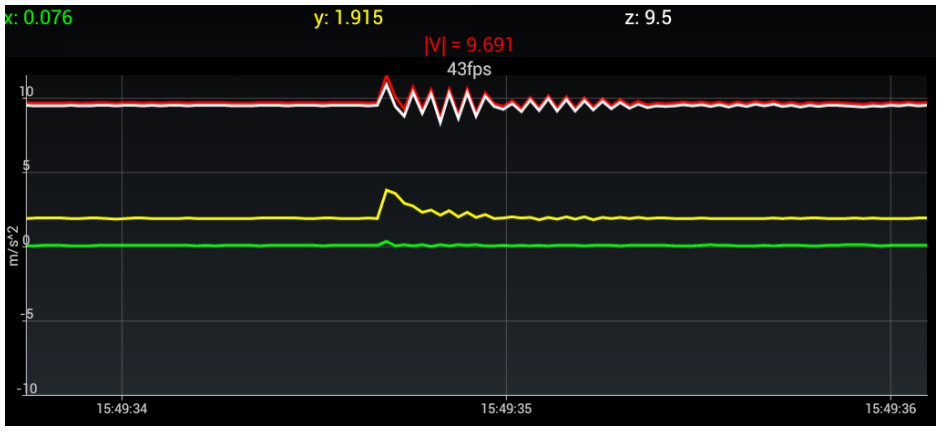
\includegraphics[width=\textwidth]{/Abstract_Chart.png}
\label{fig:Webapp_Editor}
\end{figure}
Offensichtlich werden diese Sensoren ständig ausgelöst, wenn der Benutzer das Gerät mit sich führt, während er sich fortbewegt. Dabei sind die Werte der Sensoren unmittelbar von der individuellen Bewegung abhängig und daher stets zwischen zwei Geräten verschieden.\\
Interessant wäre es, wenn es möglich wäre, Korrelationen zwischen den Sensorwerten auf verschiedenen Geräten zu finden. Dies würde darauf hindeuten, dass beide Geräte, zumal wenn sie an verschiedenen Orten aufbewahrt werden, dasselbe Ereignis wahrgenommen haben, etwa eine Erschütterung im Boden. \\
Dies könnte dazu genutzt werden, um ein automatisches Erdbebenmeldesystem zu realisieren. Wenn eine gewisse Menge von Geräten zur gleichen Zeit ein ähnliches Erschütterungsmuster detektieren, ist davon auszugehen, dass sich ein Erdbeben ereignet. Dies wird natürlich von den Anwendern selbst auch bemerkt werden, jedoch könnten die Geräte einerseits einen Alarm auslösen, der auch solche Menschen warnt, die aus diversen Gründen das Ereignis nicht wahrnehmen (schlafen oder im Auto sitzen), andererseits könnten Sicherheitsmaßnahmen in Gang gesetzt werden (automatisches Abstellen der Gasversorgung, Abstellen des Stroms an gefährlichen Orten usw.).
\newpage